% vim: set spell spelllang=en tw=100 et sw=4 sts=4 foldmethod=marker foldmarker={{{,}}} :

\documentclass{beamer}

\usepackage{tikz}
\usepackage{xcolor}
\usepackage{complexity}
\usepackage{hyperref}
\usepackage{gnuplot-lua-tikz}
\usepackage[vlined]{algorithm2e} % algorithms

\usetikzlibrary{shapes, arrows, shadows, calc, positioning, fit}
\usetikzlibrary{decorations.pathreplacing, decorations.pathmorphing, shapes.misc}
\usetikzlibrary{tikzmark}

\colorlet{screenverylightgrey}{black!2!white}
\colorlet{screengrey}{black!30!white}

\definecolor{uofgblue}{rgb}{0, 0.321569, 0.533333}
\colorlet{uofgblue20}{uofgblue!20!white}
\colorlet{uofgblue40}{uofgblue!40!white}
\colorlet{uofgblue60}{uofgblue!60!white}
\colorlet{uofgblue80}{uofgblue!80!white}

\definecolor{uofgstone}{rgb}{0.498039, 0.454902, 0.403922}

\definecolor{uofgtdarkgreen}{rgb}{0.380392, 0.564706, 0.501961}
\definecolor{uofgtlightgreen}{rgb}{0.615686, 0.788235, 0.729412}
\definecolor{uofgtyellow}{rgb}{0.85098, 0.827451, 0.643137}
\definecolor{uofgtorange}{rgb}{0.784314, 0.694118, 0.545098}

% make gnuplot graphs use our preferred choice of colours.
\colorlet{gp lt color 0}{uofgblue40}
\colorlet{gp lt color 1}{uofgblue60}
\colorlet{gp lt color 2}{uofgtlightgreen!50!white}
\colorlet{gp lt color 3}{uofgtlightgreen}
\colorlet{gp lt color 4}{uofgblue}
\colorlet{gp lt color 5}{black}
\colorlet{gp lt color 6}{uofgtdarkgreen}
\colorlet{gp lt color 7}{uofgtorange}

% {{{ theme things
\useoutertheme[footline=authorinstitutetitle]{miniframes}
\useinnertheme{rectangles}

\setbeamerfont{block title}{size={}}
\setbeamercolor*{structure}{fg=uofgblue}
\setbeamercolor*{palette primary}{use=structure,fg=black,bg=white}
\setbeamercolor*{palette secondary}{use=structure,fg=black,bg=uofgblue40}
\setbeamercolor*{palette tertiary}{use=structure,fg=white,bg=uofgblue}
\setbeamercolor*{palette quaternary}{fg=white,bg=black}

\setbeamercolor*{titlelike}{parent=palette primary}

\beamertemplatenavigationsymbolsempty

\tikzset{vertex/.style={draw, circle, inner sep=0pt, minimum size=0.5cm, font=\small\bfseries}}
\tikzset{notvertex/.style={vertex, color=white, text=black}}
\tikzset{plainvertex/.style={vertex}}
\tikzset{selectedvertex/.style={vertex, fill=uofgblue}}
\tikzset{vertexc1/.style={vertex, fill=uofgblue40}}
\tikzset{vertexc2/.style={vertex, fill=uofgblue}}
\tikzset{vertexc3/.style={vertex, fill=uofgtdarkgreen}}
\tikzset{vertexc4/.style={vertex, fill=uofgtorange}}
\tikzset{edge/.style={color=screengrey}}
\tikzset{bedge/.style={ultra thick}}
\tikzset{edgel1/.style={ultra thick, color=uofgblue}}
\tikzset{edgel2/.style={ultra thick, color=uofgblue40}}
\tikzset{edgel3/.style={ultra thick, color=uofgtdarkgreen}}
\tikzset{edgel4/.style={ultra thick, color=uofgtorange}}

\setbeamertemplate{title page}
{
    \vbox{}
    \vspace*{0.5cm}
    \begin{centering}
        {\usebeamerfont{title}\inserttitle\par}
        \vskip0.5cm\par
        \begin{beamercolorbox}[sep=8pt,center]{author}
            \usebeamerfont{author}\insertauthor
        \end{beamercolorbox}
        {\usebeamercolor[fg]{titlegraphic}\inserttitlegraphic\par}
    \end{centering}
    \vfill

    \begin{tikzpicture}[remember picture, overlay]
        \node at (current page.north west) {\begin{tikzpicture}[remember picture, overlay]\fill
        [fill=uofgblue, anchor=north west] (0, 0) rectangle (\paperwidth, -1.5cm);\end{tikzpicture}};
        \node [anchor=north west, shift={(0.2cm,-0.2cm)}] at (current page.north west) {\includegraphics*[keepaspectratio=true,scale=0.5]{UoG_keyline.eps}};
    \end{tikzpicture}
}

% }}}

\title{Phase III of the SICSA Multicore Challenge}
\author[Ciaran McCreesh]{\textcolor{uofgblue}{Ciaran McCreesh} \and Hans-Wolfgang Loidl}

\begin{document}

{
    \usebackgroundtemplate{\includegraphics*[keepaspectratio=true, height=\paperheight]{background.jpg}}
    \begin{frame}[plain]
        \titlepage
    \end{frame}
}

\begin{frame}{Multicore Challenges}
    \begin{itemize}
        \item Phase I: linear
        \item Phase II: quadratic
        \item Phase III: exponential
    \end{itemize}
\end{frame}

\begin{frame}{The Maximum Clique Problem}

    \centering
    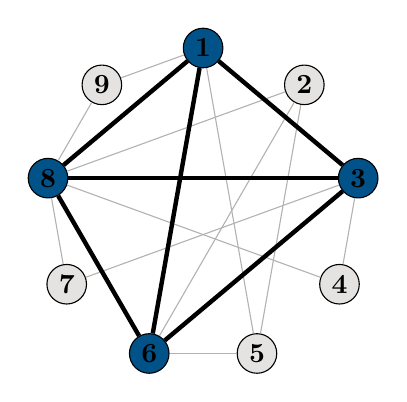
\begin{tikzpicture}%{{{
        \newcount \c
        \foreach \n in {1, ..., 9}{
            \c=\n
            \multiply\c by -40
            \advance\c by 130
            \ifthenelse{\n = 1 \OR \n = 3 \OR \n = 6 \OR \n = 8}{
                \node[draw, circle, fill=uofgblue, inner sep=2pt] (N\n) at (\the\c:2) {\textbf{\n}};
            }{
                \node[draw, circle, fill=uofgstone!20!white, inner sep=2pt] (N\n) at (\the\c:2) {\textbf{\n}};
            }
        }

        \draw [edge] (N1) -- (N5); \draw [edge] (N1) -- (N9);
        \draw [edge] (N2) -- (N5); \draw [edge] (N2) -- (N6); \draw [edge] (N2) -- (N8);
        \draw [edge] (N3) -- (N4); \draw [edge] (N3) -- (N7);
        \draw [edge] (N4) -- (N8);
        \draw [edge] (N5) -- (N6);
        \draw [edge] (N7) -- (N8);
        \draw [edge] (N8) -- (N9);

        \draw [bedge] (N1) -- (N3);
        \draw [bedge] (N6) -- (N8);
        \draw [bedge] (N1) -- (N6);
        \draw [bedge] (N1) -- (N8);
        \draw [bedge] (N3) -- (N6);
        \draw [bedge] (N3) -- (N8);
    \end{tikzpicture}%}}}
    \\~

\end{frame}

\begin{frame}{Why?}
    \begin{itemize}
        \item A competitive, well-understood sequential algorithm can fit on one page.
        \item Non-trivial (irregular, speculative), but not too difficult (no learning).
        \item Bit-parallelism is easy, and it has been task-parallelised successfully at least
            twice.
        \item We have large families of standard benchmark instances.
        \item Easy to verify implementation correctness.
        \item Ties in with the Graph500 benchmark suite.
    \end{itemize}
\end{frame}

\begin{frame}{Branch and Bound}

    \centering
    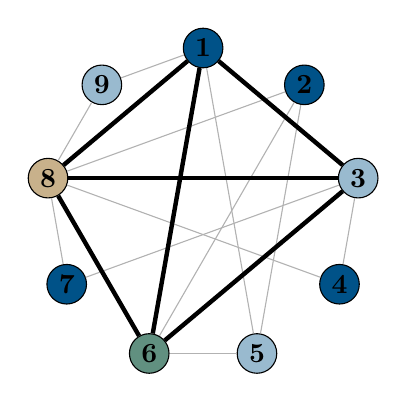
\begin{tikzpicture}%{{{
        \newcount \c
        \foreach \n in {1, ..., 9}{
            \c=\n
            \multiply\c by -40
            \advance\c by 130

            \ifthenelse{\n = 1 \OR \n = 2 \OR \n = 4 \OR \n = 7}{
                \node [draw, circle, fill=uofgblue, inner sep=2pt] (N\n) at (\the\c:2) {\textbf{\n}};
            }{
                \ifthenelse{\n = 3 \OR \n = 5 \OR \n = 4 \OR \n = 7 \OR \n = 9}{
                    \node [draw, circle, fill=uofgblue40, inner sep=2pt] (N\n) at (\the\c:2) {\textbf{\n}};
                }{
                    \ifthenelse{\n = 6}{
                        \node [draw, circle, fill=uofgtdarkgreen, inner sep=2pt] (N\n) at (\the\c:2) {\textbf{\n}};
                    }{
                        \node [draw, circle, fill=uofgtorange, inner sep=2pt] (N\n) at (\the\c:2) {\textbf{\n}};
                    }
                }
            }
        }

        \draw [edge] (N1) -- (N5); \draw [edge] (N1) -- (N9);
        \draw [edge] (N2) -- (N5); \draw [edge] (N2) -- (N6); \draw [edge] (N2) -- (N8);
        \draw [edge] (N3) -- (N4); \draw [edge] (N3) -- (N7);
        \draw [edge] (N4) -- (N8);
        \draw [edge] (N5) -- (N6);
        \draw [edge] (N7) -- (N8);
        \draw [edge] (N8) -- (N9);

        \draw [bedge] (N1) -- (N3);
        \draw [bedge] (N6) -- (N8);
        \draw [bedge] (N1) -- (N6);
        \draw [bedge] (N1) -- (N8);
        \draw [bedge] (N3) -- (N6);
        \draw [bedge] (N3) -- (N8);
    \end{tikzpicture}%}}}
    \\~

\end{frame}

\begin{frame}{Parallel Tree Search}

    \centering
    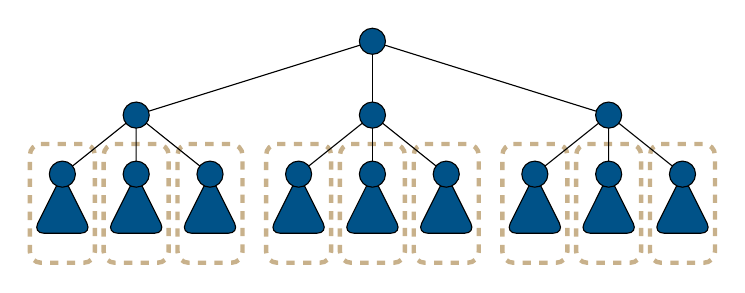
\begin{tikzpicture}[scale=0.75]%{{{
        \coordinate (R);

        \coordinate (N) at (R);

        \coordinate (N1) at ($(N) + (-4, -1.25)$);
        \coordinate (N2) at ($(N) + ( 0, -1.25)$);
        \coordinate (N3) at ($(N) + ( 4, -1.25)$);

        \foreach \na in {1, ..., 3}{
            \coordinate (N\na 1) at ($(N\na) + (-1.25, -1)$);
            \coordinate (N\na 2) at ($(N\na) + ( 0,    -1)$);
            \coordinate (N\na 3) at ($(N\na) + ( 1.25, -1)$);

            \foreach \nb in {1, ..., 3}{
                \coordinate (N\na\nb t1) at ($(N\na\nb) + (-0.5, -1)$);
                \coordinate (N\na\nb t2) at ($(N\na\nb) + ( 0.5, -1)$);
            }
        }

        \tikzstyle{p} = [draw, rounded corners, dashed, color=uofgtorange, ultra thick];
        \foreach \na in {1, ..., 3}{
            \foreach \nb in {1, ..., 3}{
                \draw [p] ($(N\na\nb) + (-0.55, 0.51)$) -- ($(N\na\nb) + (0.55, 0.51)$) --
                    ($(N\na\nb) + (0.55, -1.5)$) -- ($(N\na\nb) + (-0.55, -1.5)$) -- cycle;
                }
        }

        \foreach \na in {1, ..., 3}{
            \draw (N) -- (N\na);
            \foreach \nb in {1, ..., 3}{
                \draw (N\na) -- (N\na\nb);
            }
        }

        \tikzstyle{t} = [draw, fill, fill=uofgblue, rounded corners];
        \foreach \na in {1, ..., 3}{
            \foreach \nb in {1, ..., 3}{
                \draw [t] (N\na\nb) -- (N\na\nb t1) -- (N\na\nb t2) -- cycle;
            }
        }

        \tikzstyle{c} = [draw, circle, fill, fill=uofgblue];
        \node [c] at (N) { };

        \foreach \na in {1, ..., 3}{
            \node [c] at (N\na) { };

            \foreach \nb in {1, ..., 3}{
                \node [c] at (N\na\nb) { };
            }
        }
    \end{tikzpicture}%}}}
    \\~

\end{frame}

\begin{frame}{Anomalous Results}
    \begin{centering}
        \input{gen-graph-togian-brock400_1-speedup}
    \end{centering}
\end{frame}

\begin{frame}{Work so Far}
    \begin{itemize}
        \item \url{http://tinyurl.com/cliquepaper}
        \item \url{http://tinyurl.com/cliquewiki}
        \item Implementations in C++, Java, Haskell, Vector Pascal
    \end{itemize}
\end{frame}

\begin{frame}[b]
    \vfill
    \begin{center}
    \url{http://dcs.gla.ac.uk/~ciaran} \\
    \href{mailto:c.mccreesh.1@research.gla.ac.uk}{\nolinkurl{c.mccreesh.1@research.gla.ac.uk}}
\end{center}
\begin{tikzpicture}[remember picture, overlay]
    \node at (current page.north west) {\begin{tikzpicture}[remember picture, overlay]\fill
    [fill=uofgblue, anchor=north west] (0, 0) rectangle (\paperwidth, -1.5cm);\end{tikzpicture}};
    \node [anchor=north west, shift={(0.2cm,-0.2cm)}] at (current page.north west) {\includegraphics*[keepaspectratio=true,scale=0.5]{UoG_keyline.eps}};
\end{tikzpicture}
\end{frame}

\end{document}

